\chapter{Graph Drawing}

In this chapter, we will write \emph{iterative} methods for drawing graphs. General idea is to:
\begin{enumerate}
\item Start with a random drawing of a graph
\item Iteratively improve the drawing
\end{enumerate}

\section{Method 1: Mass center}

Write the following functions:
\begin{enumerate}
\item \verb|move_vertex_c(G, v, pos)|\\
    Where $G$ is graph, $v$ is a vertex in $G$ and $\mathrm{pos}$ is a dictionary of positions for each vertex. It should move position of $v$ to the mass center of its neighbors, i.e., $\mathrm{pos}(v) = 1/|N(v)| \sum_{u \in N(v)} \mathrm{pos}(u)$.
\item \verb|draw_graph_c(G, F, iters)|\\
    Where $G$ is graph, $F$ is a list of fixed vertices, $\mathrm{iters}$ is a number of iterations. Function should
    \begin{enumerate}
        \item Draw positions of vertices of $F$ on a circle (with radius 1, i.e., set positions of $F$ to vertices of a regular polygon).
        \item Other vertices, $V(G)\setminus F$, set to random positions in square $[-0.5, 0.5] \times [-0.5, 0.5]$.
        \item Use function \verb|move_vertex_c| to change the position of each vertex $V(G)\setminus F$.
        \item Repeat Step 3 $\mathrm{iters}$ times.
    \end{enumerate}
\end{enumerate}

\medskip
\begin{sageCell}
def move_vertex_c(G, v, pos):
    """
    Move vertex v to the mass center of its neighbors.
    """
    sx = 0
    sy = 0
    N = 0
    for u in G.neighbors(v):
        x,y = pos[u]
        sx += x
        sy += y
        N += 1
    if N > 0:
        pos[v] = (sx/N, sy/N)
\end{sageCell}
\begin{sageCell}
def draw_graph_c(G, F, iters):
    """
    Draw graph G with fixed vertices F using mass center method.
    """
    pos = {}
    for i in range(len(F)):
        pos[F[i]] = (cos(2*i*math.pi/len(F)), sin(2*i*math.pi/len(F)))
    vert = [v for v in G.vertices(sort=False) if v not in F]
    for v in vert:
        pos[v] = (random() - 0.5, random() - 0.5)
    for i in range(iters):
        for v in vert:
            move_vertex_c(G, v, pos)
    G.set_pos(pos)
    return G.plot(vertex_labels = False, vertex_size = 10)
\end{sageCell}
Example:
\begin{sageCell}
def find_cycle(G0):
    """
    An ad-hoc function to find some cycle in a graph, provided that G is 2-connected
    """
    G = G0.copy()
    e = G.edges(sort=False)[0]
    G.delete_edge(e)
    return G.shortest_path(e[0], e[1])
\end{sageCell}
\begin{sageCell}
    G = graphs.BuckyBall()
    draw_graph_c(G, find_cycle(G), 5)
\end{sageCell}

\begin{outImage}
    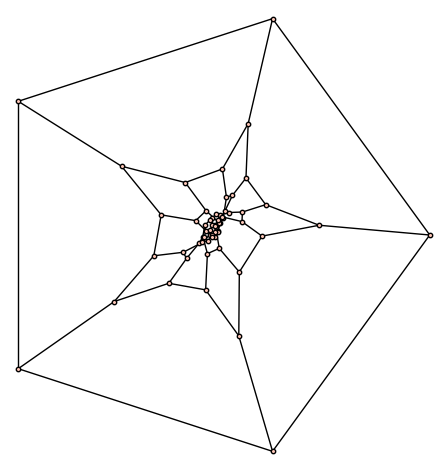
\includegraphics[width=0.5\textwidth]{Images/Drawing/bucky_ball_mass_5.png}
\end{outImage}

\begin{sageCell}
    G = graphs.BuckyBall()
    draw_graph_c(G, find_cycle(G), 100)
\end{sageCell}
\begin{outImage}
    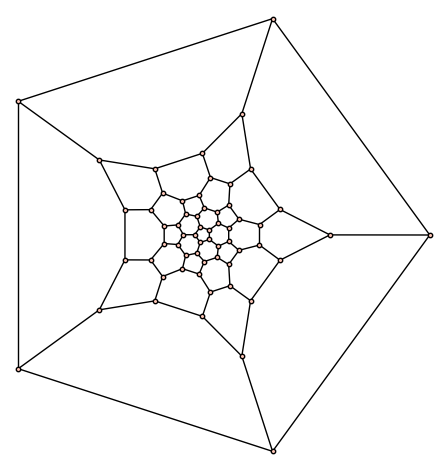
\includegraphics[width=0.5\textwidth]{Images/Drawing/bucky_ball_mass_100.png}
\end{outImage}

\section{Method 2: Move vertices using force}

Write the following functions:
\begin{enumerate}
\item \verb|move_vertex_f(G, v, pos, k)|\\
    Where $G$ is graph, $v$ is a vertex in $G$, $\mathrm{pos}$ is a dictionary of positions for each vertex and $k$ is a constant.
    Similar to \verb|move_vertex_c|, just use "forces" to move vertex $v$. Each edge $vu$ ($u$ is a neighbor of $v$) acts like a "spring" and acts with force $\vec{F} = k\: \vec{\delta}$ where $\vec{\delta} = \vec{u} - \vec{v}$ (Hooke's law) and $k$ is characteristic of the spring (razteznostni koeficient in Slovene). That is: $\mathrm{pos}(v) = \mathrm{pos}(v) + \sum_{u \in N(v)} k (\mathrm{pos}(u) - \mathrm{pos}(v))$.
\item \verb|draw_graph_f(G, F, k, iters)|\\
    which acts in the same way as \verb|draw_graph_c|, but it uses the function \verb|move_vertex_f| instead of \verb|move_vertex_c|.
\end{enumerate}

\medskip
\begin{sageCell}
def move_vertex_f(G, v, pos, k):
    """
    Move vertex v using force method.
    """
    vx, vy = pos[v]
    fx, fy = pos[v]
    for u in G.neighbors(v):
        x,y = pos[u]
        dx = x - vx
        dy = y - vy
        fx += dx * k
        fy += dy * k
    pos[v] = (fx, fy)


def draw_graph_f(G, F, k, iters):
    pos = {}
    for i in range(len(F)):
        pos[F[i]] = (cos(2*i*math.pi/len(F)), sin(2*i*math.pi/len(F)))
    vert = [v for v in G.vertices(sort=False) if v not in F]
    for v in vert:
        pos[v] = (random() - 0.5, random() - 0.5)
    for i in range(iters):
        for v in vert:
            move_vertex_f(G, v, pos, k)
    G.set_pos(pos)
    return G.plot(vertex_labels = False, vertex_size = 10)
\end{sageCell}
\begin{sageCell}
    G = graphs.BuckyBall()
    draw_graph_f(G, find_cycle(G), 0.1, 100)
\end{sageCell}
\begin{outImage}
    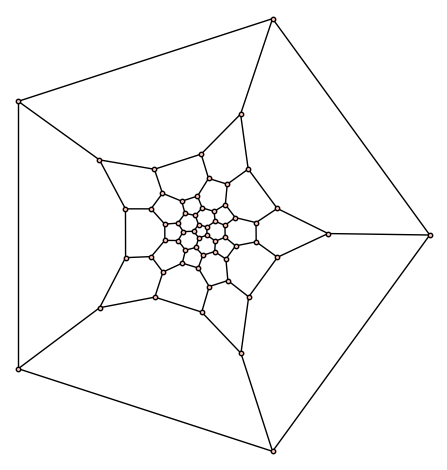
\includegraphics[width=0.5\textwidth]{Images/Drawing/bucky_ball_force_100.png}
\end{outImage}

\section{Method 3: Spring embedder}

For both methods above we required a cycle to be selected before fixing its coordinates. But this is not "practical". Can we do without this?
Without fixing some vertices, and using only the (attractive) force method, the vertices of the graph will eventually move to a single point. So we need to add \emph{repulsive} forces.

\begin{enumerate}
    \item \verb|move_vertex_se(G, v, pos, k, e)|\\
    Similar to \verb|move_vertex_f|, each edge $vu$ acts like a "spring" and acts with force $
    \vec{F} = k\: \vec{\delta}$ where $\vec{\delta} = \vec{u} - \vec{v}$. Additionally: vertices also act in a repulsive way with force $\vec{R} = -e\: \vec{\delta}/|\vec{\delta}|^2$ for all $u \neq v$. With the repulsive force we do not allow two vertices to be too close, since the force is inversely proportional to the square of the distance between them!
    \item \verb|draw_graph_se(G, k, e, iters)|\\
    Similar to \verb|draw_graph_f|, just use \verb|move_vertex_se| instead of \verb|move_vertex_f|. Note that there are no fixed vertices. Initially, for each vertex, choose a random position in the square $[-0.5, 0.5] \times [-0.5, 0.5]$.
\end{enumerate}

\medskip
\begin{sageCell}
    def move_vertex_se(G, v, pos, k, e):
    vx, vy = pos[v]
    fx, fy = pos[v]
    for u in G.neighbors(v):
        x,y = pos[u]
        dx = x - vx
        dy = y - vy
        fx += dx * k
        fy += dy * k
    for u in G.vertices(sort=False):
        if v == u:
            continue
        x, y = pos[u]
        dx = x - vx
        dy = y - vy
        r2 = dx*dx + dy*dy
        fx += -e*dx/r2
        fy += -e*dy/r2
    pos[v] = (fx, fy)


def draw_graph_se(G, k, e, iters):
    pos = {}
    for v in G.vertices(sort=False):
        pos[v] = (random() - 0.5, random() - 0.5)
    for i in range(iters):
        for v in G.vertices(sort=False):
            move_vertex_se(G, v, pos, k, e)
    G.set_pos(pos)
    return G.plot(vertex_labels = False, vertex_size = 10)
\end{sageCell}

For the graphs below, try to find $k$ and $e$ such that the result will be "nice".

\begin{sageCell}
    G = graphs.BuckyBall()
    draw_graph_se(G, ?, ?, 100)
\end{sageCell}
\begin{outImage}
    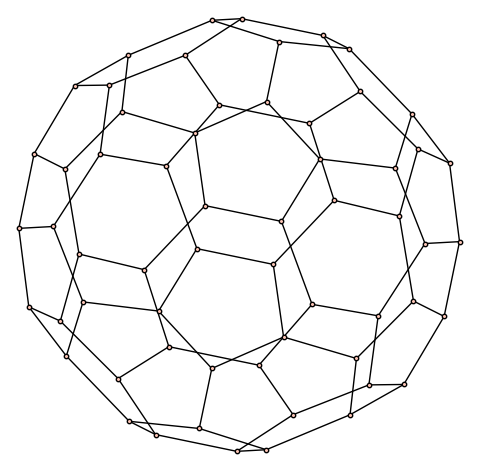
\includegraphics[width=0.5\textwidth]{Images/Drawing/bucky_ball_se_100.png}
\end{outImage}

More examples
\begin{sageCell}
    draw_graph_se(graphs.Grid2dGraph(10, 10), ?, ?, 100)

    draw_graph_se(graphs.CycleGraph(10), ?, ?, 100)

    C10 = graphs.CycleGraph(10)
    C4 = graphs.CycleGraph(4)
    draw_graph_se(C10.cartesian_product(C4), ?, ?, 100)

    draw_graph_se(graphs.RandomTree(100), ?, ?, 100)

    draw_graph_se(Graph('ShCHGD@?K?_@?@?C_GGG@??cG?G?GK_?C'), ?, ?, 100)
\end{sageCell}
